../cictikz/src/cictikz/data/tex/cictikz_preamble.tex

% Gate-source voltage applied: the gate energy shifts down by qV, some
% voltage drops across the oxide (drawn tilted), and the bands in the
% bulk bend down towards the surface.

\definecolor{lblred}{RGB}{160,25,35}
\definecolor{eblue}{RGB}{85,155,235}

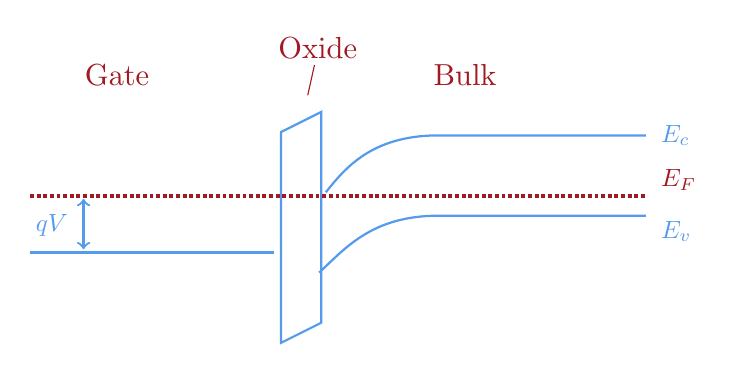
\begin{tikzpicture}[scale=0.85]

  % oxide: the interfaces stay vertical, only the band edges tilt
  % with the field across the oxide
  \draw[eblue, thick] (4.05,-0.7) -- (4.05,2.45) -- (4.65,2.75) -- (4.65,-0.4) -- cycle;

  % gate level, pulled down by qV
  \draw[eblue, thick] (0.3,0.65) -- (3.95,0.65);
  \draw[lblred, densely dotted, line width=1.4pt] (0.3,1.5) -- (9.5,1.5);
  \node[lblred, anchor=south west, scale=0.9] at (9.6,1.45) {$E_F$};
  \draw[eblue, thick, <->] (1.1,0.7) -- (1.1,1.45);
  \node[eblue, anchor=east, scale=0.9] at (1.0,1.05) {$qV$};

  % bulk bands bending down towards the surface
  \draw[eblue, thick]
    (9.5,2.4) -- (6.4,2.4) .. controls (5.4,2.4) and (5.0,1.9) .. (4.72,1.55);
  \node[eblue, anchor=west, scale=0.9] at (9.6,2.4) {$E_c$};
  \draw[eblue, thick]
    (9.5,1.2) -- (6.4,1.2) .. controls (5.4,1.2) and (5.0,0.7) .. (4.62,0.35);
  \node[eblue, anchor=north west, scale=0.9] at (9.6,1.25) {$E_v$};

  % region labels
  \node[lblred, anchor=center, scale=1.1] at (1.6,3.3) {Gate};
  \node[lblred, anchor=center, scale=1.1] at (4.6,3.7) {Oxide};
  \draw[lblred, thin] (4.55,3.45) -- (4.45,3.0);
  \node[lblred, anchor=center, scale=1.1] at (6.8,3.3) {Bulk};

\end{tikzpicture}
\end{document}
